\documentclass[journal,12pt,onecolumn]{IEEEtran}
\usepackage{cite}
\usepackage{graphicx}
\usepackage{amsmath,amssymb,amsfonts,amsthm}
\usepackage{algorithmic}
\usepackage{graphicx}
\usepackage{textcomp}
\usepackage{xcolor}
\usepackage{txfonts}
\usepackage{listings}
\usepackage{enumitem}
\usepackage{mathtools}
\usepackage{gensymb}
\usepackage{comment}
\usepackage[breaklinks=true]{hyperref}
\usepackage{tkz-euclide} 
\usepackage{listings}
\usepackage{gvv}                                        
%\def\inputGnumericTable{}                                 
\usepackage[latin1]{inputenc} 
\usetikzlibrary{arrows.meta, positioning}
\usepackage{xparse}
\usepackage{color}                                            
\usepackage{array}                                            
\usepackage{longtable}                                       
\usepackage{calc}                                             
\usepackage{multirow}
\usepackage{multicol}
\usepackage{hhline}                                           
\usepackage{ifthen}                                           
\usepackage{lscape}
\usepackage{tabularx}
\usepackage{array}
\usepackage{float}
\newtheorem{theorem}{Theorem}[section]
\newtheorem{problem}{Problem}
\newtheorem{proposition}{Proposition}[section]
\newtheorem{lemma}{Lemma}[section]
\newtheorem{corollary}[theorem]{Corollary}
\newtheorem{example}{Example}[section]
\newtheorem{definition}[problem]{Definition}
\newcommand{\BEQA}{\begin{eqnarray}}
\newcommand{\EEQA}{\end{eqnarray}}
\usepackage{float}
%\newcommand{\define}{\stackrel{\triangle}{=}}
\theoremstyle{remark}
\usepackage{circuitikz}
\usepackage{tikz}

\title{IN: INSTRUMENTATION ENGINEERING}
\author{EE25BTECH11031- Sai Sreevallabh}

\author{Sai Sreevallabh - ee25btech11031}

\begin{document}

\maketitle

\section*{\textbf{Q.1-Q.20 Carry one mark each}} 

\begin{enumerate}
%1
\item If $z=x+jy$, where $x$ and $y$ are real, the value of $|e^{jz}|$ is \par \hfill\brak{\text{GATE IN 2009}}
    \begin{enumerate}
    \begin{multicols}{4}
        \item $1$
        \item $e^{\sqrt{{x^{2}+y^{2}}}}$
        \item $e^{y}$
        \item $e^{-y}$
\end{multicols}
\end{enumerate}

%2
\item The value of $\oint\frac{sinz}{z}dz$, where the contour of integration is a simple closed curve around the origin, is \par \hfill\brak{\text{GATE IN 2009}} 
\begin{enumerate}
    \begin{multicols}{4}
        \item $0$
        \item $2{\pi}j$
        \item $\infty$
        \item $1/\brak{2{\pi}j}$
\end{multicols}
\end{enumerate}

%3
\item Let  $\textbf{P} \not= \textbf{0}$ be a $3 \times 3$ real matrix. There exist linearly independent vectors $\Vec{x}$ and $\Vec{y}$ such that $\textbf{P}\vec{x} = 0$ and $\textbf{P}\vec{y} = 0$. The dimension of the range space of \textbf{P} is \par \hfill\brak{\text{GATE IN 2009}}
\begin{enumerate}
    \begin{multicols}{4}
        \item $0$
        \item $1$
        \item $2$
        \item $3$
\end{multicols}
\end{enumerate}

%4
\item A sphere of unit radius is centered at the origin. The unit normal at a point $\brak{x,y,z}$ on the surface of the sphere is the vector \par \hfill\brak{\text{GATE IN 2009}}
\begin{enumerate}
    \begin{multicols}{4}
        \item $\brak{x,y,z}$
        \item $\brak{\frac{1}{\sqrt{3}},\frac{1}{\sqrt{3}},\frac{1}{\sqrt{3}}}$
        \item $\brak{\frac{x}{\sqrt{3}},\frac{y}{\sqrt{3}},\frac{z}{\sqrt{3}}}$
        \item $\brak{\frac{x}{\sqrt{2}},\frac{y}{\sqrt{2}},\frac{z}{\sqrt{2}}}$
\end{multicols}
\end{enumerate}


 
%5
\item An LVDT is supplied with a sinusoidal voltage of amplitude $5V$ and frequency $1\text{kH}$. The output is connected to an ac voltmeter. The reading of the voltmeter is $1V$ for a displacement of $1\text{mm}$ from the null position. When the displacement is $1\text{mm}$ in the opposite direction from the null position, the reading of the voltmeter is \par \hfill\brak{\text{GATE IN 2009}}
\begin{enumerate}
    \begin{multicols}{4}
        \item -$1\text{V}$
        \item $-0.2\text{V}$
        \item $1\text{V}$
        \item $5\text{V}$
\end{multicols}
\end{enumerate}

 
%6
\item The circuit shown in $\figref{fig:placeholder_1}$ is
\begin{figure}[H]
    \centering
    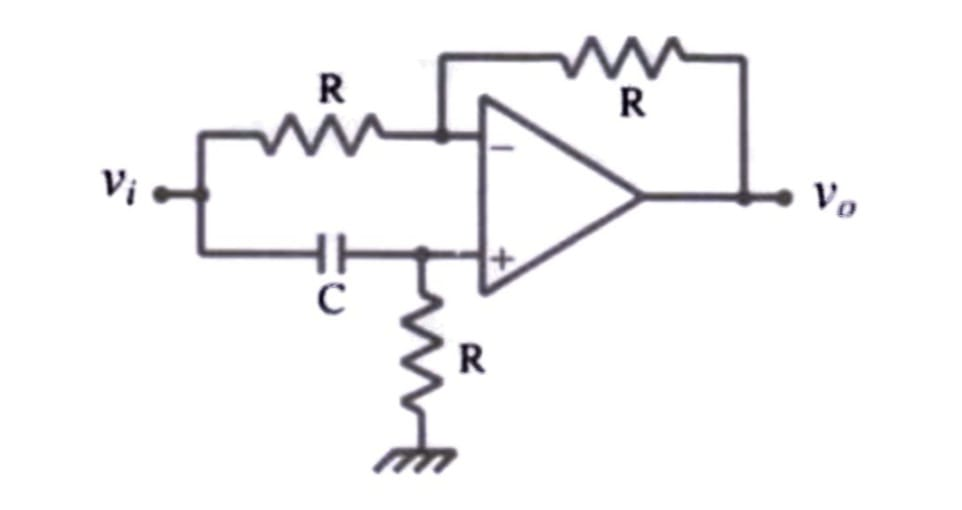
\includegraphics[width=0.3\columnwidth]{Figs/Q-6.jpg}
    \caption{Circuit Diagram}
    \label{fig:placeholder_1}
\end{figure}
. \hfill\brak{\text{GATE IN 2009}}
\begin{enumerate}
   \begin{multicols}{2}
       \item an all-pass filter
       \item a bandpass filter
       \item a highpass filter
       \item a lowpass filter
   \end{multicols}
\end{enumerate}

 
%7
\item The diodes shown in the circuit ($\figref{fig:placeholder_2}$) are ideal. A voltage of $0V$ represents logic $0$ and $+5V$  represents logic $1$. The logic function Z realized by the circuit for logic inputs X and Y is\par  \hfill\brak{\text{GATE IN 2009}}
\begin{figure}[H]
    \centering
    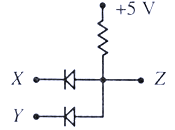
\includegraphics[width=0.3\columnwidth]{Figs/Q-7.png}
    \caption{Circuit Diagram}
    \label{fig:placeholder_2}
\end{figure}
\begin{enumerate}
    \begin{multicols}{2}
        \item $Z=X+Y$
        \item $Z=XY$
        \item $Z=\overline{X+Y}$
        \item $Z=\overline{XY}$
\end{multicols}
\end{enumerate}

 
%8
\item The minimal sum-of-products expression for the logic function $f$ represented by the given Karnaugh map (\figref{fig:placeholder_3}) is\par \hfill\brak{\text{GATE IN 2009}} 
\begin{figure}[H]
    \centering
    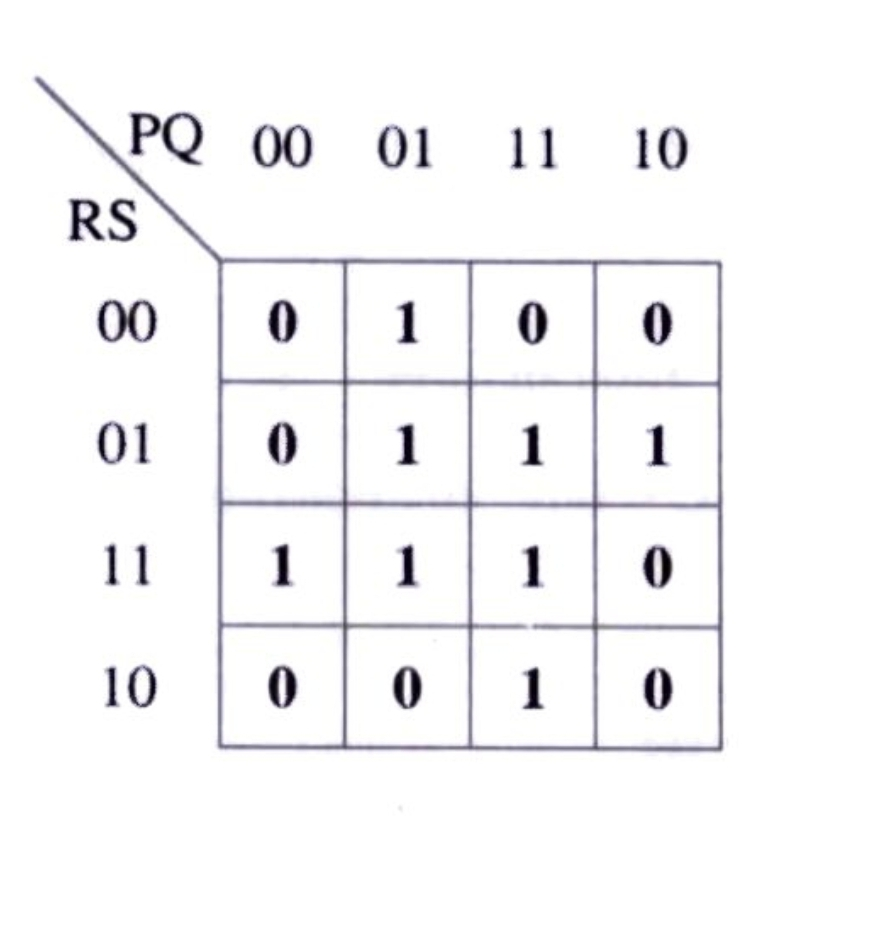
\includegraphics[width=0.3\columnwidth]{Figs/Q-8.jpg}
    \caption{Karnaugh map}
    \label{fig:placeholder_3}
\end{figure}
    \begin{enumerate}
        \item $QS+P\overline{R}S+PQR+\overline{P}RS+\overline{P}Q\overline{R}$
        \item $\overline{QS}+\overline{P}R\overline{S}+\bar{P}\bar{Q}R+\overline{P}\overline{R}S+P\overline{Q}R$
        \item $\overline{P}R\overline{S}+\bar{P}\bar{Q}\bar{R}+P\bar{R}\bar{S}+P\overline{Q}R$
        \item $P\overline{R}S+PQR+\overline{P}RS+\overline{P}Q\overline{R}$
\end{enumerate}

 
%9
\item In \figref{fig:placeholder_4}, the initial state of $Q$ is $0$. The output is observed after the application of each clock pulse. The output sequence at $Q$ is\par \hfill\brak{\text{GATE IN 2009}}
\begin{figure}[H]
    \centering
    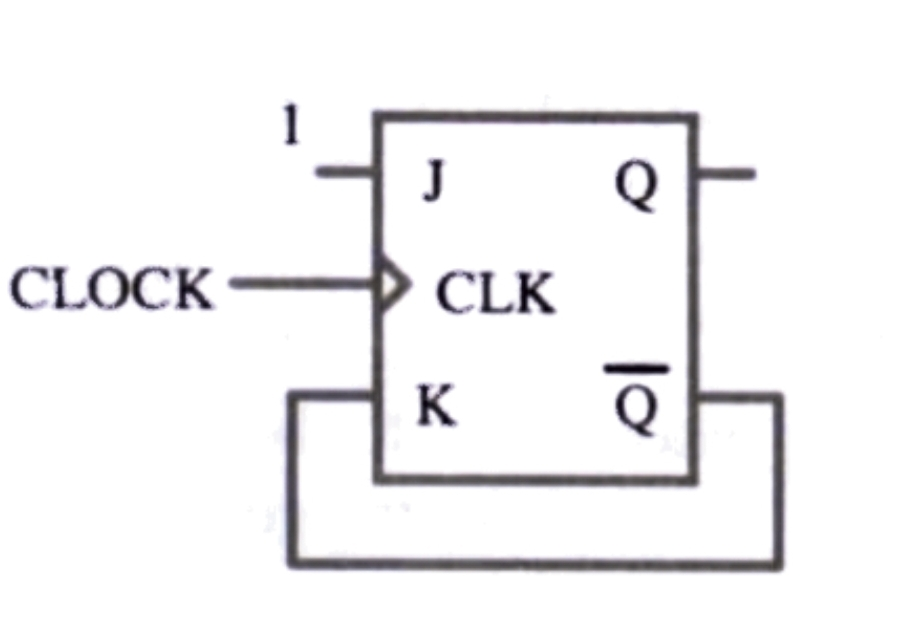
\includegraphics[width=0.3\columnwidth]{Figs/Q-9.jpg}
    \caption{For Question-9}
    \label{fig:placeholder_4}
\end{figure}
\begin{enumerate}
    \begin{multicols}{4}
        \item $0000\dots$
        \item $1010\dots$
        \item $1111\dots$
        \item $1000\dots$
\end{multicols}
\end{enumerate}

 
%10
\item The binary representation of the decimal number $1.375$ is\par \hfill\brak{\text{GATE IN 2009}}
\begin{enumerate}
    \begin{multicols}{2}
        \item $1.111$
        \item $1.010$
        \item $1.011$
        \item $1.001$
\end{multicols}
\end{enumerate}

%11
\item Consider a system consisting of microprocessor, memory and peripheral devices connected by a common bus. During DMA data transfer, the microprocessor\par \hfill\brak{\text{GATE IN 2009}}
    \begin{enumerate}
        \item only reads from the bus
        \item only writes to the bus
        \item both reads from and writes to the bus
        \item neither reads from nor writes to the bus
\end{enumerate}

 
%12
\item The fundamental period of $x\brak{t}=2\sin{2{\pi}t} + 3\sin3{\pi}t$, with $t$ expressed in seconds, is\par \hfill\brak{\text{GATE IN 2009}}
\begin{enumerate}
    \begin{multicols}{4}
        \item $1\text{s}$
        \item $0.67\text{s}$
        \item $2\text{s}$
        \item $3\text{s}$
\end{multicols}
\end{enumerate}

 
%13
\item A linear time-invariant causal system has a frequency response given in polar form as $\frac{1}{\sqrt{1+{\omega}^2}}$$\angle-tan^{-1}\omega$. For input $x\brak{t}=\sin{t}$, the output is  \par \hfill\brak{\text{GATE IN 2009}}
\begin{enumerate}
    \begin{multicols}{4}
        \item $\frac{1}{\sqrt{2}}\cos{t}$
        \item $\frac{1}{\sqrt{2}}\cos{\brak{t-\frac{\pi}{4}}}$
        \item $\frac{1}{\sqrt{2}}\sin{t}$
        \item $\frac{1}{\sqrt{2}}\sin{\brak{t-\frac{\pi}{4}}}$
\end{multicols}
\end{enumerate}

 
%14
\item A $50\%$ duty cycle square wave with zero mean is used as a baseband signal in an ideal frequency modulator with a sinusoidal carrier of frequency $\omega_c$. The modulated signal is given as an input to an ideal phase demodulator (a circuit that produces an output proportional to the difference in phase of the modulated signal from that of the carrier). The output of the circuit is\par \hfill\brak{\text{GATE IN 2009}}
    \begin{enumerate}
        \item a square wave
        \item a train of impulses with alternating signs
        \item a triangular wave
        \item a sinusoidal wave
\end{enumerate}
%15
 

\item \figref{fig:placeholder_5} shows a periodic waveform to be displayed on a CRO. A trigger setting which ensures a stationary display is\par \hfill\brak{\text{GATE IN 2009}}
\begin{figure}[H]
    \centering
    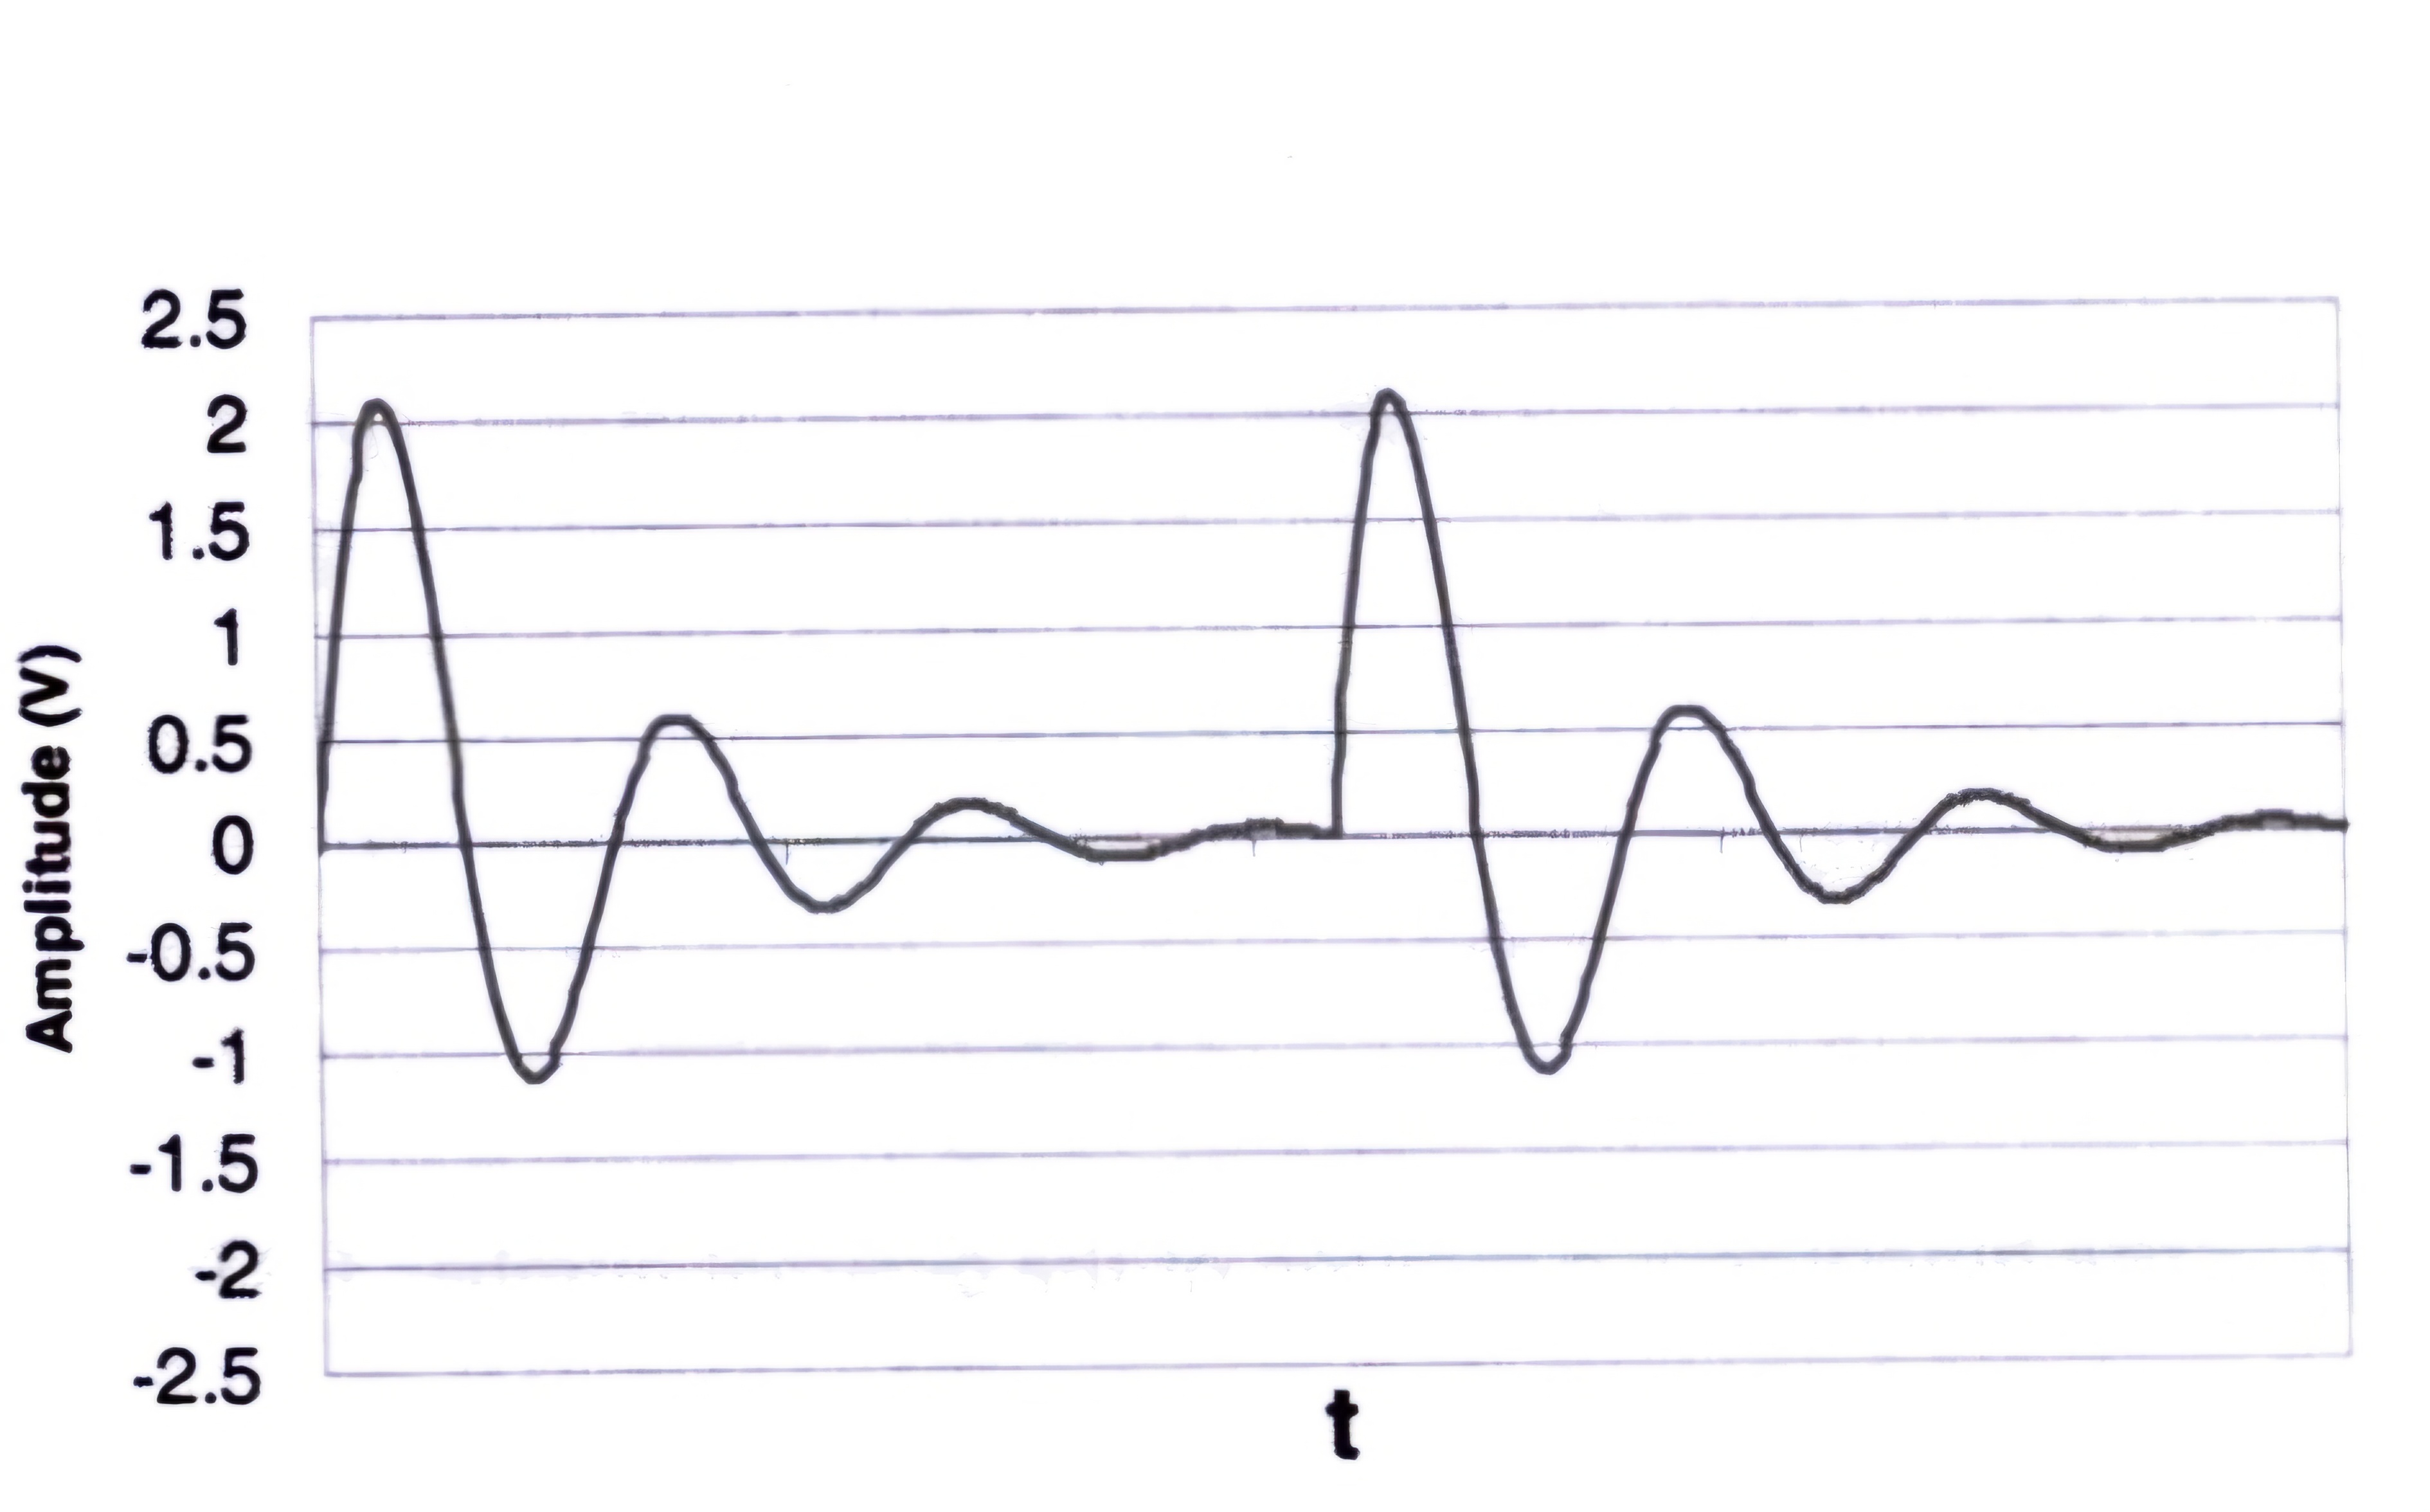
\includegraphics[width=0.5\columnwidth]{Figs/Q-15.jpg}
    \caption{Waveform}
    \label{fig:placeholder_5}
\end{figure}
\begin{enumerate}
    \begin{multicols}{2}
        \item level: $0.2\text{V}$, slope: $-$ve
        \item level: $0.5\text{V}$, slope: $-$ve
        \item level: $-0.2\text{V}$, slope: $+$ve
        \item level: $1.8\text{V}$, slope: $-$ve
\end{multicols}
\end{enumerate}

 
%16
\item The input impedance of a CRO is equivalent to a $1\text{M}\ohm$ resistance in parallel with a $45\text{pF}$ capacitance. It is used with a compensated $10$-to-$1$ attenuation probe. The effective input capacitance at the probe tip is \par \hfill\brak{\text{GATE IN 2009}}
\begin{enumerate}
    \begin{multicols}{2}
        \item $4.5\text{pF}$
        \item $5\text{pF}$
        \item $45\text{pF}$
        \item $450\text{pF}$
\end{multicols}
\end{enumerate}

 
%17
\item A galvanometer with internal resistance $100\ohm$ and full-scale current $1mA$ is used to realize a dc voltmeter with a full scale range of $1\text{V}$. The full scale range of this voltmeter can be extended to $10V$ by connecting an external resistance of value \par \hfill\brak{\text{GATE IN 2009}}
\begin{enumerate}
    \begin{multicols}{2}
        \item $9\text{k}\ohm$
        \item $9.9\text{k}\ohm$
        \item $10\text{k}\ohm$
        \item $11\text{k}\ohm$
\end{multicols}
\end{enumerate}

 
%18
\item A plant with a transfer function $\frac{2}{s\brak{s+3}}$ is controlled by a PI controller with $K_p=1$ and $K_i\ge0$ in a unity feedback configuration. The lowest value of $K_i$ that ensures zero steady state error for a step change in the reference input is \par \hfill\brak{\text{GATE IN 2009}}
\begin{enumerate}
    \begin{multicols}{2}
        \item $0$
        \item $1/3$
        \item $1/2$
        \item $1$
\end{multicols}
\end{enumerate}

 
%19
\item A mass spectrometer is used to resolve peaks corresponding to $\mathrm{CO^{+}}$ and $\mathrm{N_2}^+$. The atomic masses are $^{12}\mathrm{C}=12.0000$, $^{16}\mathrm{O}=15.9949$ and $^{14}\mathrm{N}=14.0031 amu$. The resolving power of the mass spectrometer should be atleast \par \hfill\brak{\text{GATE IN 2009}}
\begin{enumerate}
    \begin{multicols}{2}
        \item $250$ 
        \item $350$
        \item $2500$
        \item $3500$
\end{multicols}
\end{enumerate}

 
%20
\item Assuming complete dissociation, the pH of a $1\text{mM}$ solution of $\mathrm{H_2SO_4}$ is closest to \par \hfill\brak{\text{GATE IN 2009}}
\begin{enumerate}
    \begin{multicols}{2}
        \item $3$
        \item $2.7$
        \item $2.4$
        \item $2.1$
\end{multicols}
\end{enumerate}

 

\section*{\textbf{Q.$21$ to Q.$60$ carry two marks each}}

 
%21
\item The eigenvalues of a $\brak{2\times2}$ matrix \textbf{X} are $-2$ and $-3$. The eigenvalues of the matrix $\brak{\textbf{X}+\textbf{I}}^{-1}\brak{\textbf{X}+5\textbf{I}}$ are \par \hfill{\brak{\text{GATE IN 2009}}}
\begin{enumerate} 
    \begin{multicols}{4}
        \item $-3, -4$
        \item $-1,-2$
        \item $-1,-3$
        \item $-2,-4$
\end{multicols}
\end{enumerate}

 
%22
\item The matrix \textbf{P} \myvec{0&0&0\\1&0&0\\0&1&0}
 rotates a vector about the axis \myvec{1\\1\\1} by an angle of \par \hfill{\brak{\text{GATE IN 2009}}}
\begin{enumerate}
    \begin{multicols}{4}
        \item $30\degree$
        \item $60\degree$
        \item $90\degree$
        \item $120\degree$
\end{multicols}
\end{enumerate}

 
%23
\item A screening test is carried out to detect a certain disease. It is found that $12\%$ of the positive reports and $15\%$ of the negative reports are incorrect. Assuming that the probability of a person getting a positive report is $0.01$, the probability that a person tested gets an incorrect report is \par \hfill{\brak{\text{GATE IN 2009}}}
\begin{enumerate}
    \begin{multicols}{4}
        \item $0.0027$
        \item $0.0173$
        \item $0.1497$
        \item $0.2100$
\end{multicols}
\end{enumerate}

 
%24
\item One of the roots of the equation $x^3=j$, where $j$ is the positive square root of $-1$, is \par \hfill{\brak{\text{GATE IN 2009}}}
\begin{enumerate}
    \begin{multicols}{4}
        \item $j$
        \item $\frac{\sqrt3}{2}+j\frac{1}{2}$
        \item $\frac{\sqrt3}{2}-j\frac{1}{2}$
        \item $-\frac{\sqrt3}{2}-j\frac{1}{2}$
\end{multicols}
\end{enumerate}

 
%25
\item The differential equation $\frac{dx}{dt}=\frac{4-x}{\tau}$ with $x\brak{0}=0$, and the constant $\tau>0$, is to be numerically integrated using the forward Euler method with a constant integration time step $T$. The maximum value of $T$ such that the numerical solution of $x$ converges is \hfill{\brak{\text{GATE IN 2009}}}
\begin{enumerate}
    \begin{multicols}{4}
        \item ${\tau}/{4}$
        \item $\tau/2$
        \item $\tau$
        \item $2\tau$
\end{multicols}
\end{enumerate}

 
%26
\item A quantity $x$ is calculated by using the formula\par
$x=\brak{p-q}/r$,\par
The measured values are $p=9$, $q=6$, $r=0.5$.\par
Assume that the measurement errors in $p,q$ and $r$ are independent. The absolute maximum error in the measurement of each of the three quantities is $\epsilon$. The absolute maximum error in the calculated value of $x$ is \par \hfill{\brak{\text{GATE IN 2009}}}
\begin{enumerate}
    \begin{multicols}{4}
        \item $\epsilon$
        \item $2\epsilon$
        \item $3\epsilon$
        \item $16\epsilon$
\end{multicols}
\end{enumerate}

 
%27
\item The response of a first order measurement system to a unit step input is $1-e^{-0.5t}$, where $t$ is in seconds. A ramp of $0.1$ units per second is given as the input to this system. The error in the measured value after transients have dies down is \par \hfill{\brak{\text{GATE IN 2009}}}
\begin{enumerate}
    \begin{multicols}{4}
        \item $0.02$ units
        \item $0.1$ units
        \item $0.2$ units
        \item $1$ unit
\end{multicols}
\end{enumerate}

 
%28
\item The source network S is connected to the load network L as shown by dashed lines (in \figref{fig:placeholder_6}). \par
The power transferred from S to L would be maximum when $R_L$ is \par \hfill{\brak{\text{GATE IN 2009}}}
\begin{figure}[H]
    \centering
    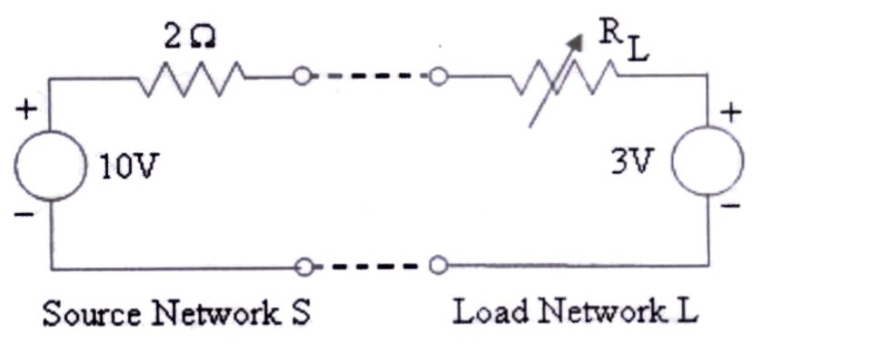
\includegraphics[width=0.5\columnwidth]{Figs/Q-28.jpg}
    \caption{Circuit Diagram}
    \label{fig:placeholder_6}
\end{figure}
\begin{enumerate}
    \begin{multicols}{4}
        \item $0\ohm$ 
        \item $0.6\ohm$
        \item $0.8\ohm$
        \item $2\ohm$ 
\end{multicols}
\end{enumerate}
%29
\item A stroboscopic system is used for measuring the speed of a rotating shaft. The shaft has one target mark on it. The maximum strobe rate at which synchronism is achieved is $r_1$ flashes per minute. The next lower flash rate at which synchronism is achieved is $r_2$ flashes per minute. The speed of the shaft in rpm is: \par \hfill{\brak{\text{GATE IN 2009}}}
\begin{enumerate}
    \begin{multicols}{4}
        \item $\frac{r_1r_2}{r_1-r_2}$
        \item $\frac{r_1r_2}{r_1+r_2}$
        \item $\frac{r_2^2}{r_1+r_2}$
        \item $\frac{r_1^2}{r_1+r_2}$
\end{multicols}
\end{enumerate}

 
%30
\item \figref{fig:placeholder_7} shows the cross-sectional diagram of an orifice flow meter with an orifice radius $R$. Point 'a' is $30\mathrm{R}$ upstream while points 'b' and 'c' are $0.8R$ and $30R$ downstream from the orifice respectively. The pressures at points a,b and c are $P_a$, $P_b$ and $P_c$ respectively. Then \par \hfill{\brak{\text{GATE IN 2009}}}
\begin{figure}[H]
    \centering
    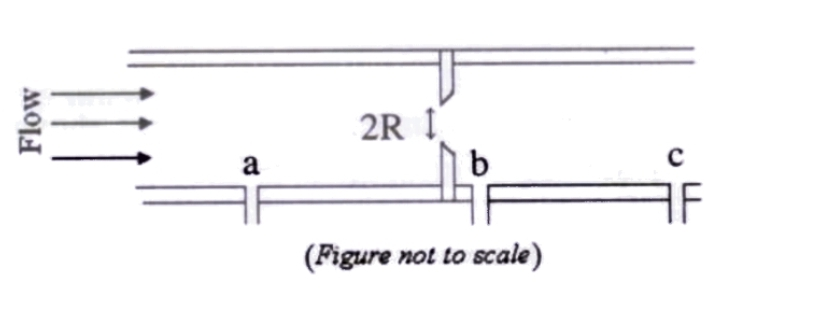
\includegraphics[width=0.5\columnwidth]{Figs/Q-30.jpg}
    \caption{Cross-sectional Diagram of an orifice flow meter}
    \label{fig:placeholder_7}
\end{figure}

\begin{enumerate}
    \begin{multicols}{2}
        \item $P_c>P_b>P_a$
        \item $P_b>P_c>P_a$
        \item $P_a>P_b>P_c$
        \item $P_a>P_c>P_b$
\end{multicols}
\end{enumerate}

 
%31
\item The values of the material constant $\beta$ for the thermistors P and Q are $4000\text{K}$ and $3000\text{K}$, respectively. The resistance of each thermistor at $298\text{K}$ is $2\text{k}\ohm$. At $373\text{K}$, the ratio of the resistance of thermistor P to that of thermistor Q will be closest to \par \hfill{\brak{\text{GATE IN 2009}}}
\begin{enumerate}
    \begin{multicols}{2}
        \item $1.33$
        \item $1.00$
        \item $0.75$
        \item $0.50$
\end{multicols}
\end{enumerate}

 
%32
\item Four strain gauges are fixed on a cylindrical shaft to measure torque, as shown in \figref{fig:placeholder_8}\begin{figure}[H]
    \centering
    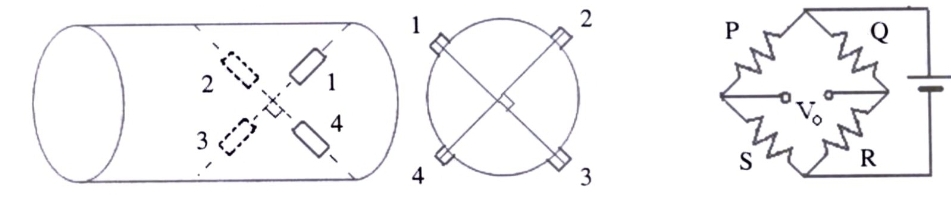
\includegraphics[width=0.9\columnwidth]{Figs/Q-32.jpg}
    \caption{Strain Gauges fixed on a Cylindrical Shaft}
    \label{fig:placeholder_8}
\end{figure} 
A correct way to place these gauges in the bridge is: \par \hfill{\brak{\text{GATE IN 2009}}}
\begin{enumerate}
    \begin{multicols}{2}
        \item P-$1$, Q-$2$, R-$3$, S-$4$
        \item P-$1$, Q-$3$, R-$2$, S-$4$
        \item P-$3$, Q-$1$, R-$2$, S-$4$
        \item P-$2$, Q-$1$, R-$3$, S-$4$
\end{multicols}
\end{enumerate}

 

%33
\item In the circuit shown in \figref{fig:placeholder_9}, the Zener diode has ideal characteristics and a breakdown voltage of $3.2\text{V}$.The output voltage $V_o$ for an input voltage $V_i=+1V$ is closest to \par \hfill{\brak{\text{GATE IN 2009}}}
\begin{figure}[H]
    \centering
    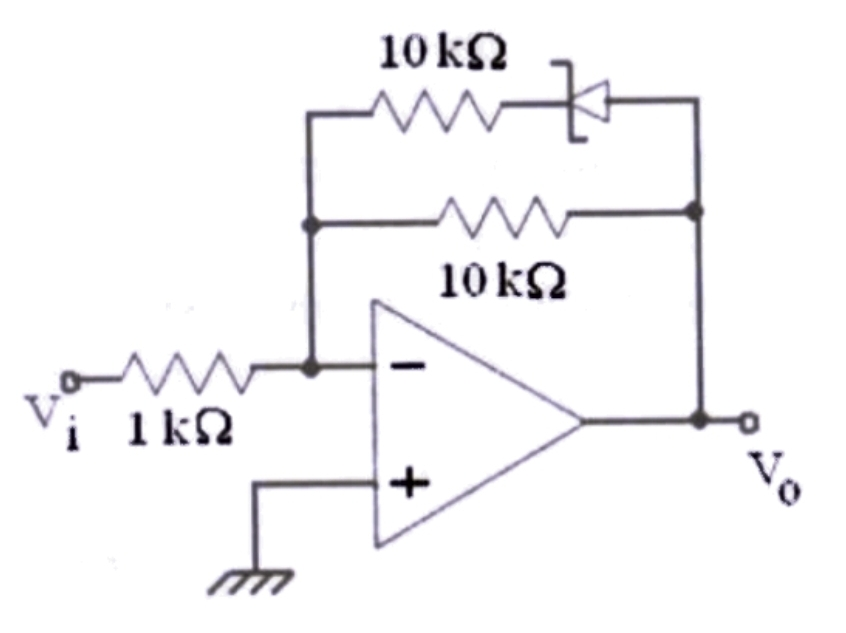
\includegraphics[width=0.3\columnwidth]{Figs/Q-33.jpg}
    \caption{Circuit Diagram}
    \label{fig:placeholder_9}
\end{figure}
\begin{enumerate}
    \begin{multicols}{2}
        \item $-10\text{V}$
        \item $-6.6\text{V}$
        \item $-5\text{V}$
        \item $-3.2\text{V}$
\end{multicols}
\end{enumerate} 

 

%34
\item The input resistance of the circuit shown in \figref{fig:placeholder_10}, assuming an ideal op amp, is \par \hfill{\brak{\text{GATE IN 2009}}}
\begin{figure}[H]
    \centering
    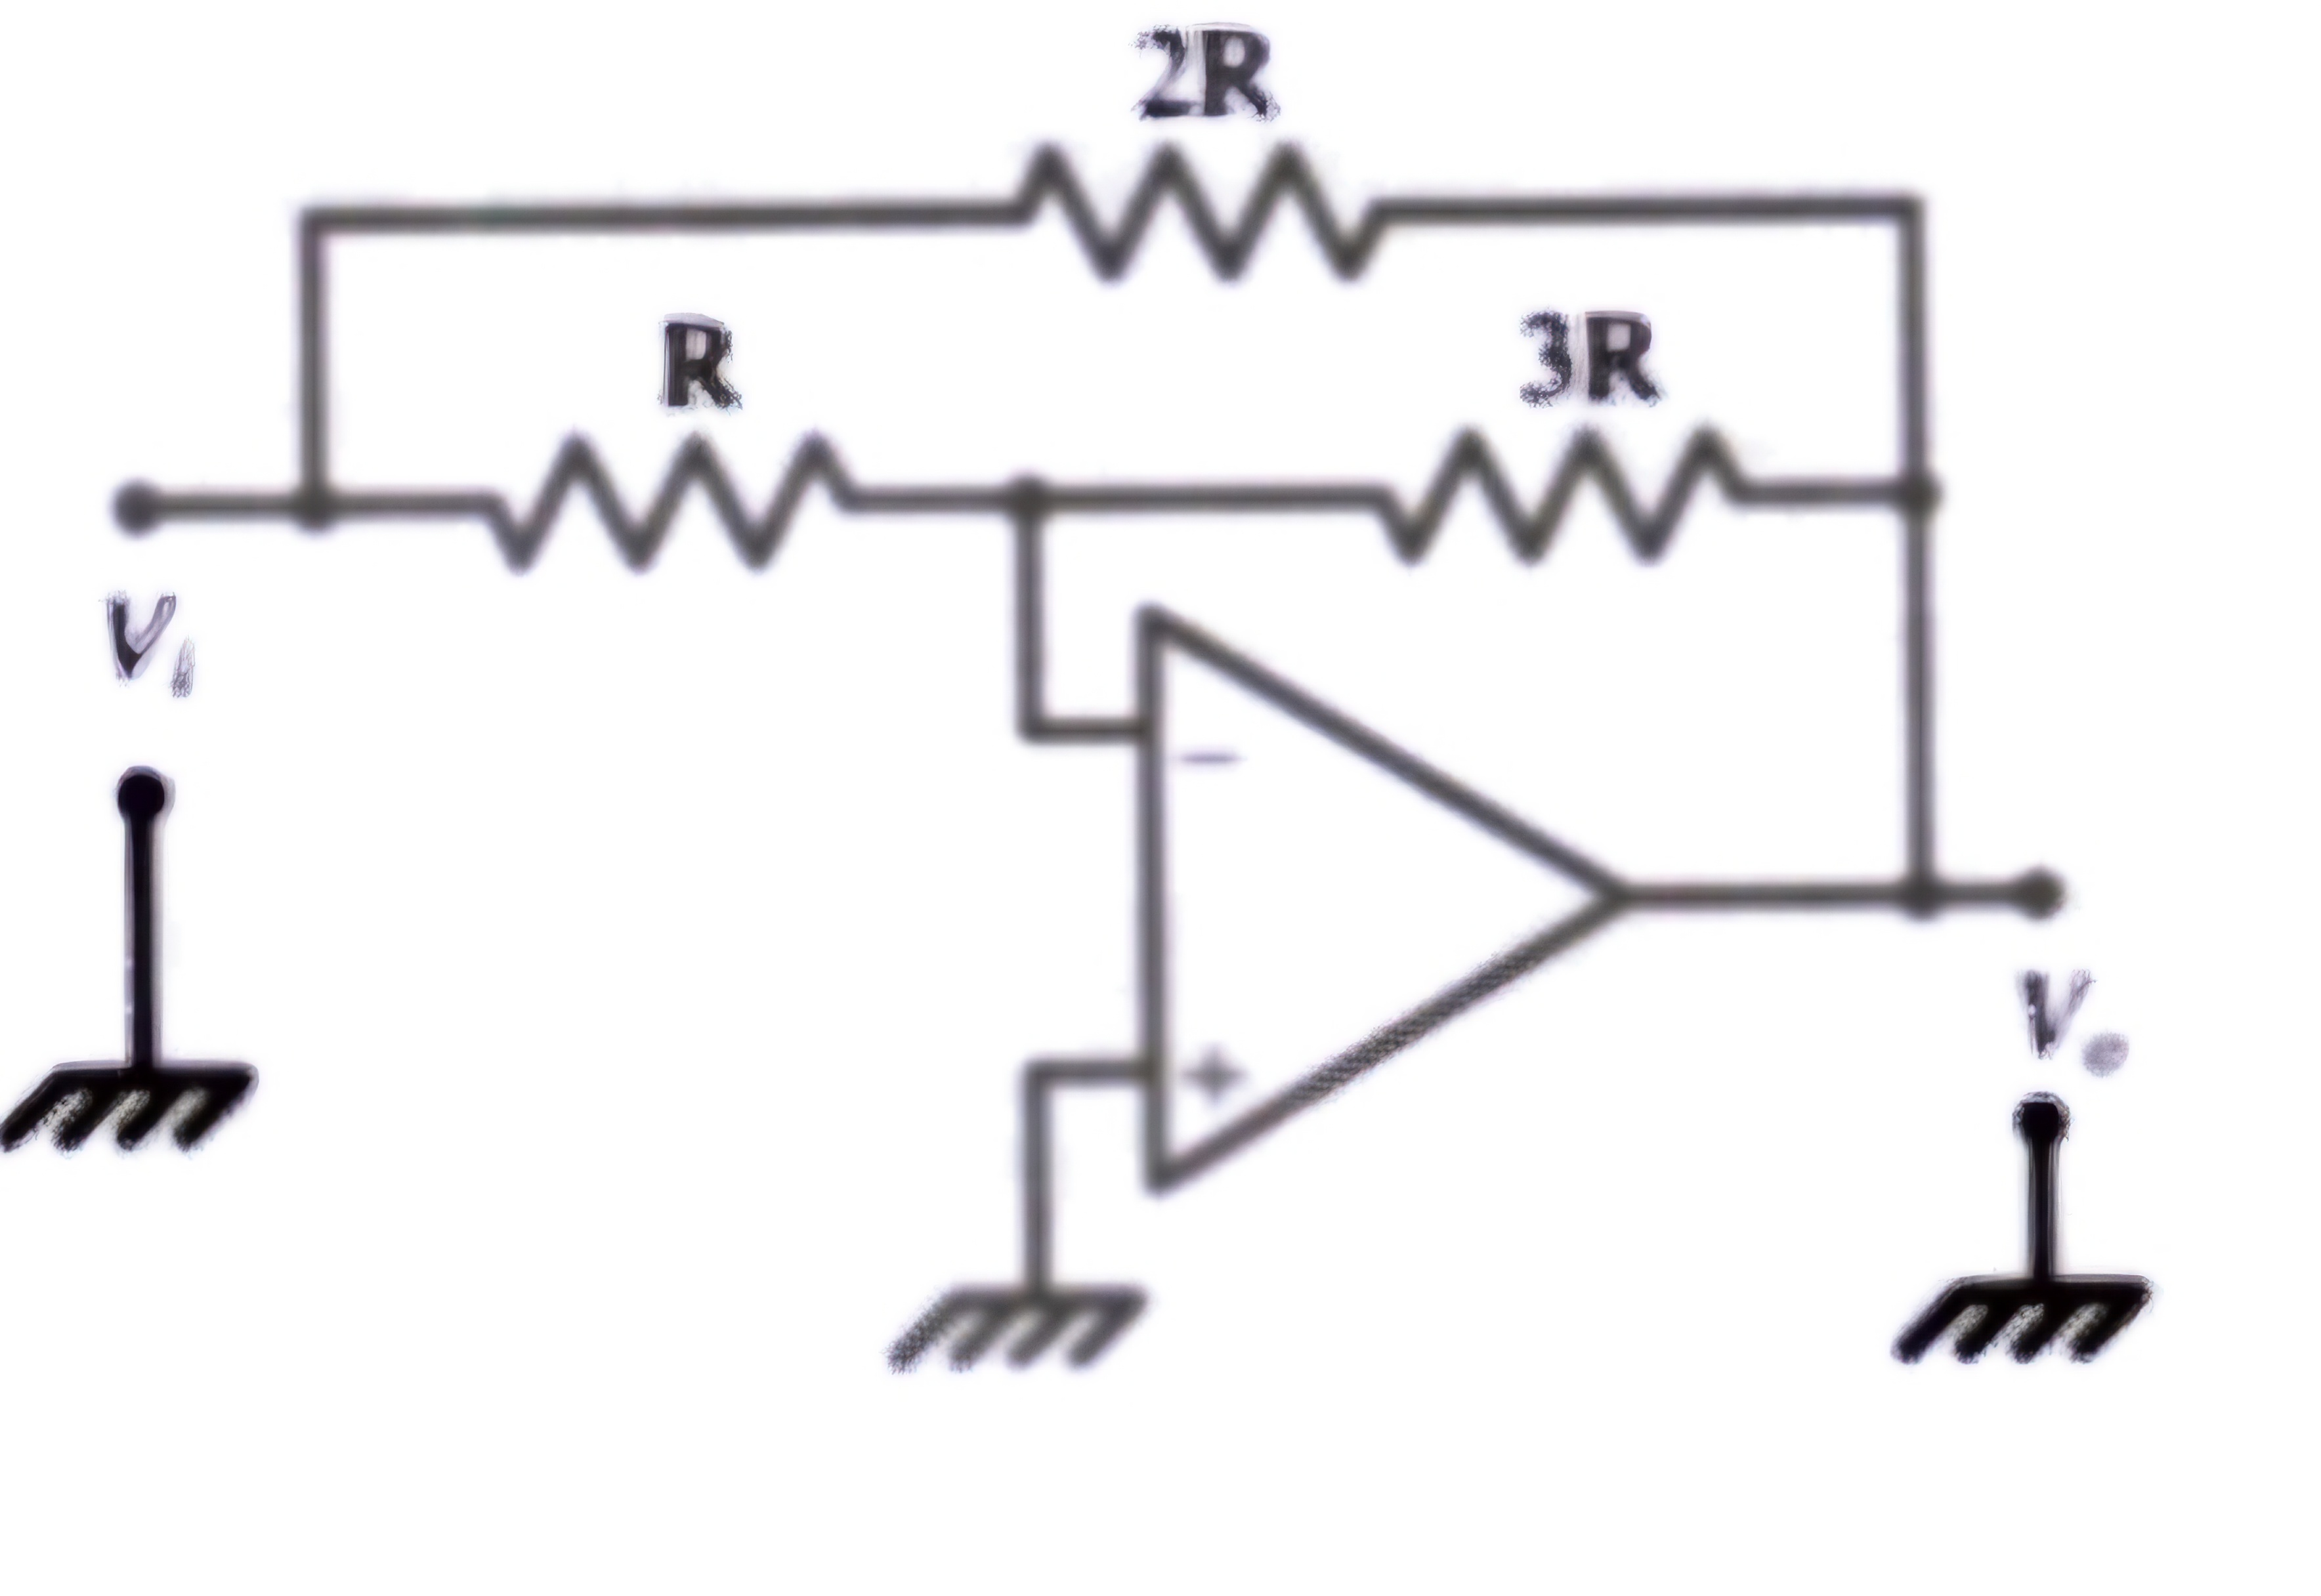
\includegraphics[width=0.3\columnwidth]{Figs/Q-34.jpg}
    \caption{Circuit Diagram}
    \label{fig:placeholder_10}
\end{figure}
\begin{enumerate}
    \begin{multicols}{2}
        \item $\text{R}/3$
        \item $2\text{R}/3$
        \item $\text{R}$
        \item $4\text{R}/3$
\end{multicols}
\end{enumerate} 

 

%35
\item In the circuit shown in \figref{fig:placeholder_11}, the switch S has been in Position $1$ for a long time. It is then moved to Position $2$. Assume the Zener diodes to be ideal. The time delay between the switch moving to Position $2$ and the transition in the output voltage $V_o$ is \par \hfill{\brak{\text{GATE IN 2009}}}
\begin{figure}[H]
    \centering
    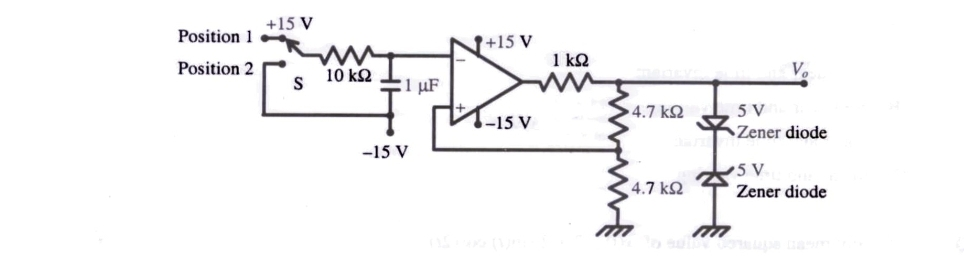
\includegraphics[width=0.9\columnwidth]{Figs/Q-35.jpg}
    \caption{Circuit Diagram}
    \label{fig:placeholder_11}
\end{figure} 
\begin{enumerate}
    \begin{multicols}{2}
        \item $5.00\text{ms}$
        \item $8.75\text{ms}$
        \item $10.00\text{ms}$
        \item $13.75\text{ms}$
\end{multicols}
\end{enumerate} 

 

%36
\item .
\begin{figure}[H]
    \centering
    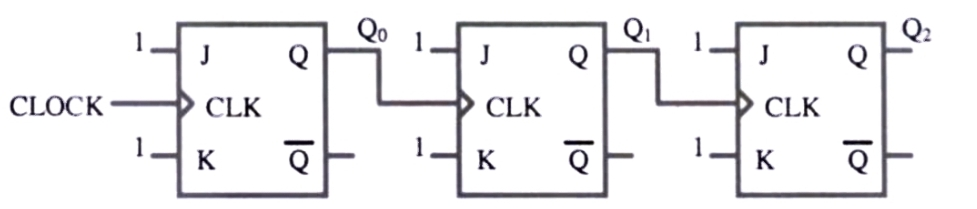
\includegraphics[width=0.5\columnwidth]{Figs/Q-36.jpg}
    \caption{Circuit Diagram}
    \label{fig:placeholder_12}
\end{figure}
\figref{fig:placeholder_12} above shows a $3$-bit ripple counter, with $Q_2$ as the MSB. The flip-flops are rising edge-triggered. The counting direction is \par  \hfill{\brak{\text{GATE IN 2009}}}
    \begin{enumerate}
        \item always down
        \item always up
        \item up or down depending on initial state of $Q_0$ only
        \item up or down depending on the initial states of $Q_2$, $Q_1$ and $Q_0$ 
\end{enumerate}

 

%37
\item An $8$-bit ADC with $2$'s complement output, has a nominal input range of $-2\text{V}$ to $+2$V. It generates a digital code of $00$H for an analog input in the range $-7.8125\text{mV}$ to $+7.8125\text{mV}$. An input of $-1.5\text{V}$ will produce a digital output of \par  \hfill{\brak{\text{GATE IN 2009}}}
\begin{enumerate}
    \begin{multicols}{4}
        \item $90$H
        \item $96$H
        \item $9$BH
        \item A$0$H
\end{multicols}
\end{enumerate} 

 

%38
\item The following is an assembly language program for $8085$ microprocessors
\begin{multicols}{3}
    \underline{Address}\\\\
    $1000$H\\
    $1002$H\\
    $1004$H\\
    $1007$H\\
    $1008$H
    
    \columnbreak
    
    \underline{Instruction Code}\\\\
    $3$E $06$\\
    C$6$ $70$\\
    $32$ $07$ $10$\\
    AF\\
    $76$
    
    \columnbreak
    
    \underline{Mnemonic}\\\\
    MVI   A, $06$H\\
    ADI   $70$H\\
    STA   $1007$H\\
    XRA   A\\
    HLT\\   
\end{multicols}
 When this program halts, the accumulator contains \par \hfill{\brak{\text{GATE IN 2009}}}
\begin{enumerate}
    \begin{multicols}{4}
        \item $00$H
        \item $06$H
        \item $70$H
        \item $76$H
\end{multicols}
\end{enumerate} 

 

%39
\item For the input $x\brak{t}$, an ideal impulse sampling system produces the output\\ $y\brak{t}=\sum_{k=-\infty}^{\infty}x\brak{kT}\delta\brak{t-kT}$, where $\delta\brak{t}$ is the Dirac delta function.\\ The system is \par  \hfill{\brak{\text{GATE IN 2009}}}
    \begin{enumerate}
        \item nonlinear and time invariant
        \item nonlinear and time varying
        \item linear and time invariant
        \item linear and time varying
\end{enumerate} 

 

%40
\item The root mean squared value of $x\brak{t}=3+2\sin\brak{t}\cos\brak{2t}$ \par  \hfill{\brak{\text{GATE IN 2009}}}
\begin{enumerate}
    \begin{multicols}{4}
        \item $\sqrt{3}$
        \item $\sqrt{8}$
        \item $\sqrt{10}$
        \item $\sqrt{11}$
\end{multicols}
\end{enumerate} 

 

%41
\item An analog signal is sampled at $9\text{kHz}$. The sequence so obtained is filtered by an FIR filter with transfer function $H[z]=1-z^{-6}$. One of the analog frequencies for which the magnitude response of the filter is zero is \par  \hfill{\brak{\text{GATE IN 2009}}}
\begin{enumerate}
    \begin{multicols}{4}
        \item $0.75\text{kHz}$
        \item $1\text{kHz}$
        \item $1.5\text{kHz}$
        \item $2\text{kHz}$
\end{multicols}
\end{enumerate} 

 

%42
\item The transfer function $H\brak{z}$ of a fourth-order linear phase FIR system is given by\\ $H\brak{z}=\brak{1+2z^{-1}+3z^{-2}}G\brak{z}$.\\
Then $G\brak{z}$ is\par  \hfill{\brak{\text{GATE IN 2009}}}
\begin{enumerate}
    \begin{multicols}{4}
        \item $3+2z^{-1}+z^{-2}$
        \item $1+\frac{1}{2}z^{-1}+\frac{1}{3}z^{-2}$
        \item $\frac{1}{3}^{-1}+2z^{-1}+z^{-2}$
        \item $1+2z+3z^{2}$
\end{multicols}
\end{enumerate} 

 
%43
\item The dc potentiometer shown in the figure has a working current of $10\text{mA}$ with switch S open. Let $R_g+R_1=100\ohm$. The galvanometer G can only detect currents greater than $10\mu{\text{A}}$. The maximum percentage error in the measurement of the unknown emf $E_x$ as calculated from the slider position shown in \figref{fig:placeholder_13} is closest to  \par  \hfill{\brak{\text{GATE IN 2009}}}
\begin{figure}[H]
    \centering
    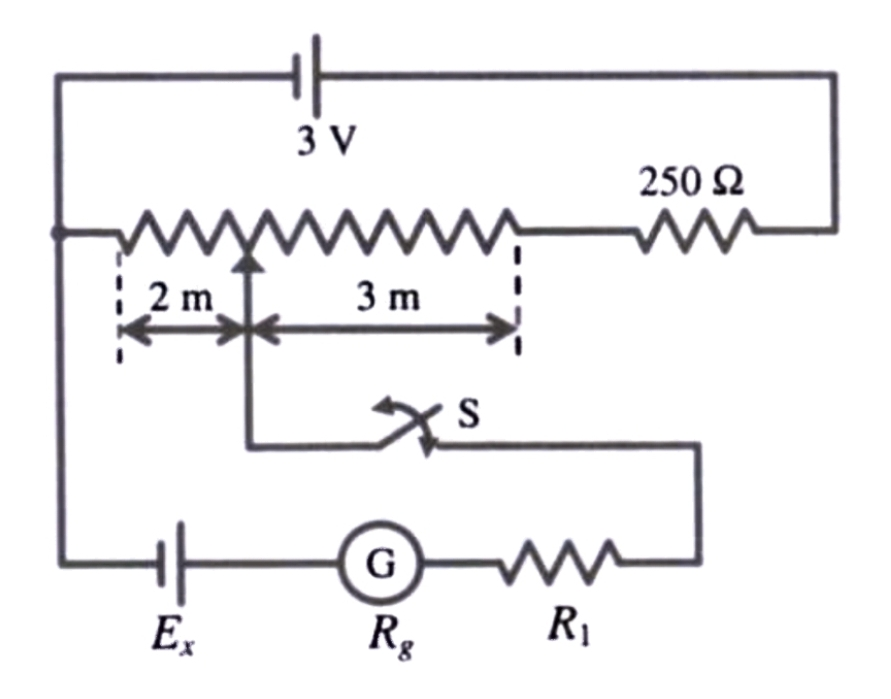
\includegraphics[width=0.4\columnwidth]{Figs/Q-43.jpg}
    \caption{DC Potentiometer}
    \label{fig:placeholder_13}
\end{figure}
\begin{enumerate}
    \begin{multicols}{4}
        \item $0.3$
        \item $0.5$
        \item $0.6$
        \item $1.0$
\end{multicols}
\end{enumerate} 

 

%44
\item A filter is represented by the signal flow graph shown in \figref{fig:placeholder_14}. Its input is $x\brak{t}$ and output is $y\brak{t}$. The transfer function of the filter is \par  \hfill{\brak{\text{GATE IN 2009}}}
\begin{figure}[H]
    \centering
    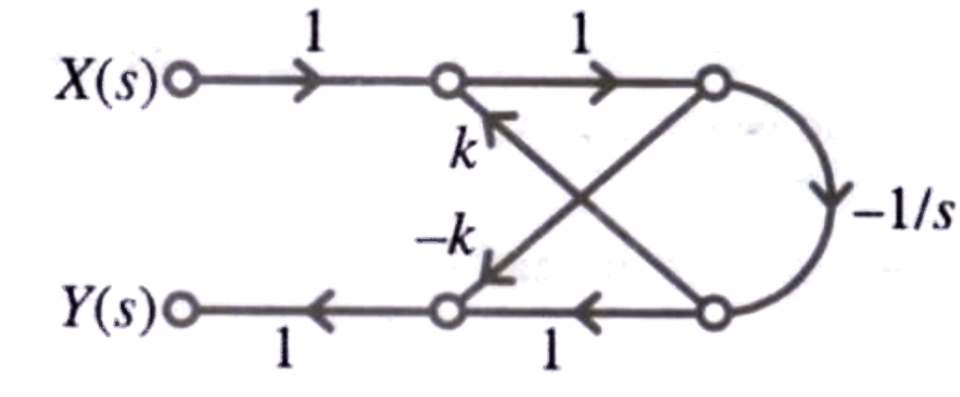
\includegraphics[width=0.5\columnwidth]{Figs/Q-44.jpg}
    \caption{Signal flow graph}
    \label{fig:placeholder_14}
\end{figure} \par
\begin{enumerate}
    \begin{multicols}{2}
        \item $\frac{-\brak{1+ks}}{s+k}$
        \item $\frac{\brak{1+ks}}{s+k}$
        \item $\frac{-\brak{1-ks}}{s+k}$
        \item $\frac{\brak{1-ks}}{s+k}$
\end{multicols}
\end{enumerate} 

 

%45
\item A unity feedback control loop with an open loop transfer function of the form $\frac{K}{s\brak{s+a}}$ has a gain crossover frequency of $1$ rad/s and a phase margin of $60\degree$. If an element having a transfer function $\frac{s-\sqrt{3}}{s+\sqrt{3}}$ is inserted into the loop, the phase margin will become \par \hfill{\brak{\text{GATE IN 2009}}}
\begin{enumerate}
    \begin{multicols}{4}
        \item $0\degree$
        \item $30\degree$
        \item $45\degree$
        \item $60\degree$
\end{multicols}
\end{enumerate} 

 

%46
\item A linear time-invariant single-input single-output system has a state space model given by \\

\begin{align}
  \frac{d\textbf{x}}{dt} & =\textbf{Fx}+\textbf{G}u\\
y= & \textbf{Hx}
\end{align}
where $\textbf{F}= \myvec{0&1\\-4&-2}
 ; \textbf{G}= \myvec{0\\1}; \textbf{H}= \myvec{1&0}$.  

 \par
 Here $\vec{x}$ is the state vector, $u$ is the input and $y$ is the output. \\
The damping ratio of the system is \par \hfill{\brak{\text{GATE IN 2009}}}
\begin{enumerate}
    \begin{multicols}{4}
        \item $0.25$
        \item $0.5$
        \item $1$
        \item $2$
\end{multicols}
\end{enumerate} 

 

%45
\item A unity feedback system has the transfer function\par

$$\frac{K\brak{s+b}}{s^2\brak{s+20}}$$\par

The value of $b$ for which the loci of all the three roots of the closed loop characteristic equation meet at a single point is \par \hfill{\brak{\text{GATE IN 2009}}}
\begin{enumerate}
    \begin{multicols}{4}
        \item $\frac{10}{9}$
        \item $\frac{20}{9}$
        \item $\frac{30}{9}$
        \item $\frac{40}{9}$
\end{multicols}
\end{enumerate} 

 

%48
\item A standard three-lead frontal plane ECG is taken with a normal heart. The peak amplitude of the R-wave is \par \hfill{\brak{\text{GATE IN 2009}}}
\begin{enumerate}
        \item greatest in lead $\mathrm{I}$
        \item greatest in lead $\mathrm{II}$
        \item greatest in lead $\mathrm{III}$
        \item equal in all the leads
\end{enumerate} 

 

%49
\item The operating voltage of an X-ray tube is changed from $40\text{kV}$ to $50\text{kV}$. The resulting change in the shortest wavelength generated is \par \hfill{\brak{\text{GATE IN 2009}}}
\begin{enumerate}
    \begin{multicols}{4}
        \item $+20\%$
        \item $-20\%$
        \item $+25\%$
        \item $-36\%$
\end{multicols}
\end{enumerate}

 

%50
\item In a pulsed ultrasound imaging system, a single $5\text{MHz}$ crystal is used both as source and as detector. Bursts of at least $20$ cycles are needed for acceptable image quality. The velocity of sound in the tissue being imaged is $1500\text{m/s}$. The minimum distance of the objects to be imaged should be \par \hfill{\brak{\text{GATE IN 2009}}}
\begin{enumerate}
    \begin{multicols}{4}
        \item $12\text{mm}$
        \item $6\text{mm}$
        \item $3\text{mm}$
        \item $1\text{mm}$
\end{multicols}
\end{enumerate}


\section*{\textbf{Common Data Questions}}


\textbf{Common Data for Questions $51$ to $52$}\par

\figref{fig:placeholder_15} shows a sample-and-hold circuit using a MOSFET as a switch. The threshold voltage of the MOSFET is $+2\text{V}$. It has zero leakage current in the off state. Assume that the capacitor is ideal.

\begin{figure}[H]
    \centering
    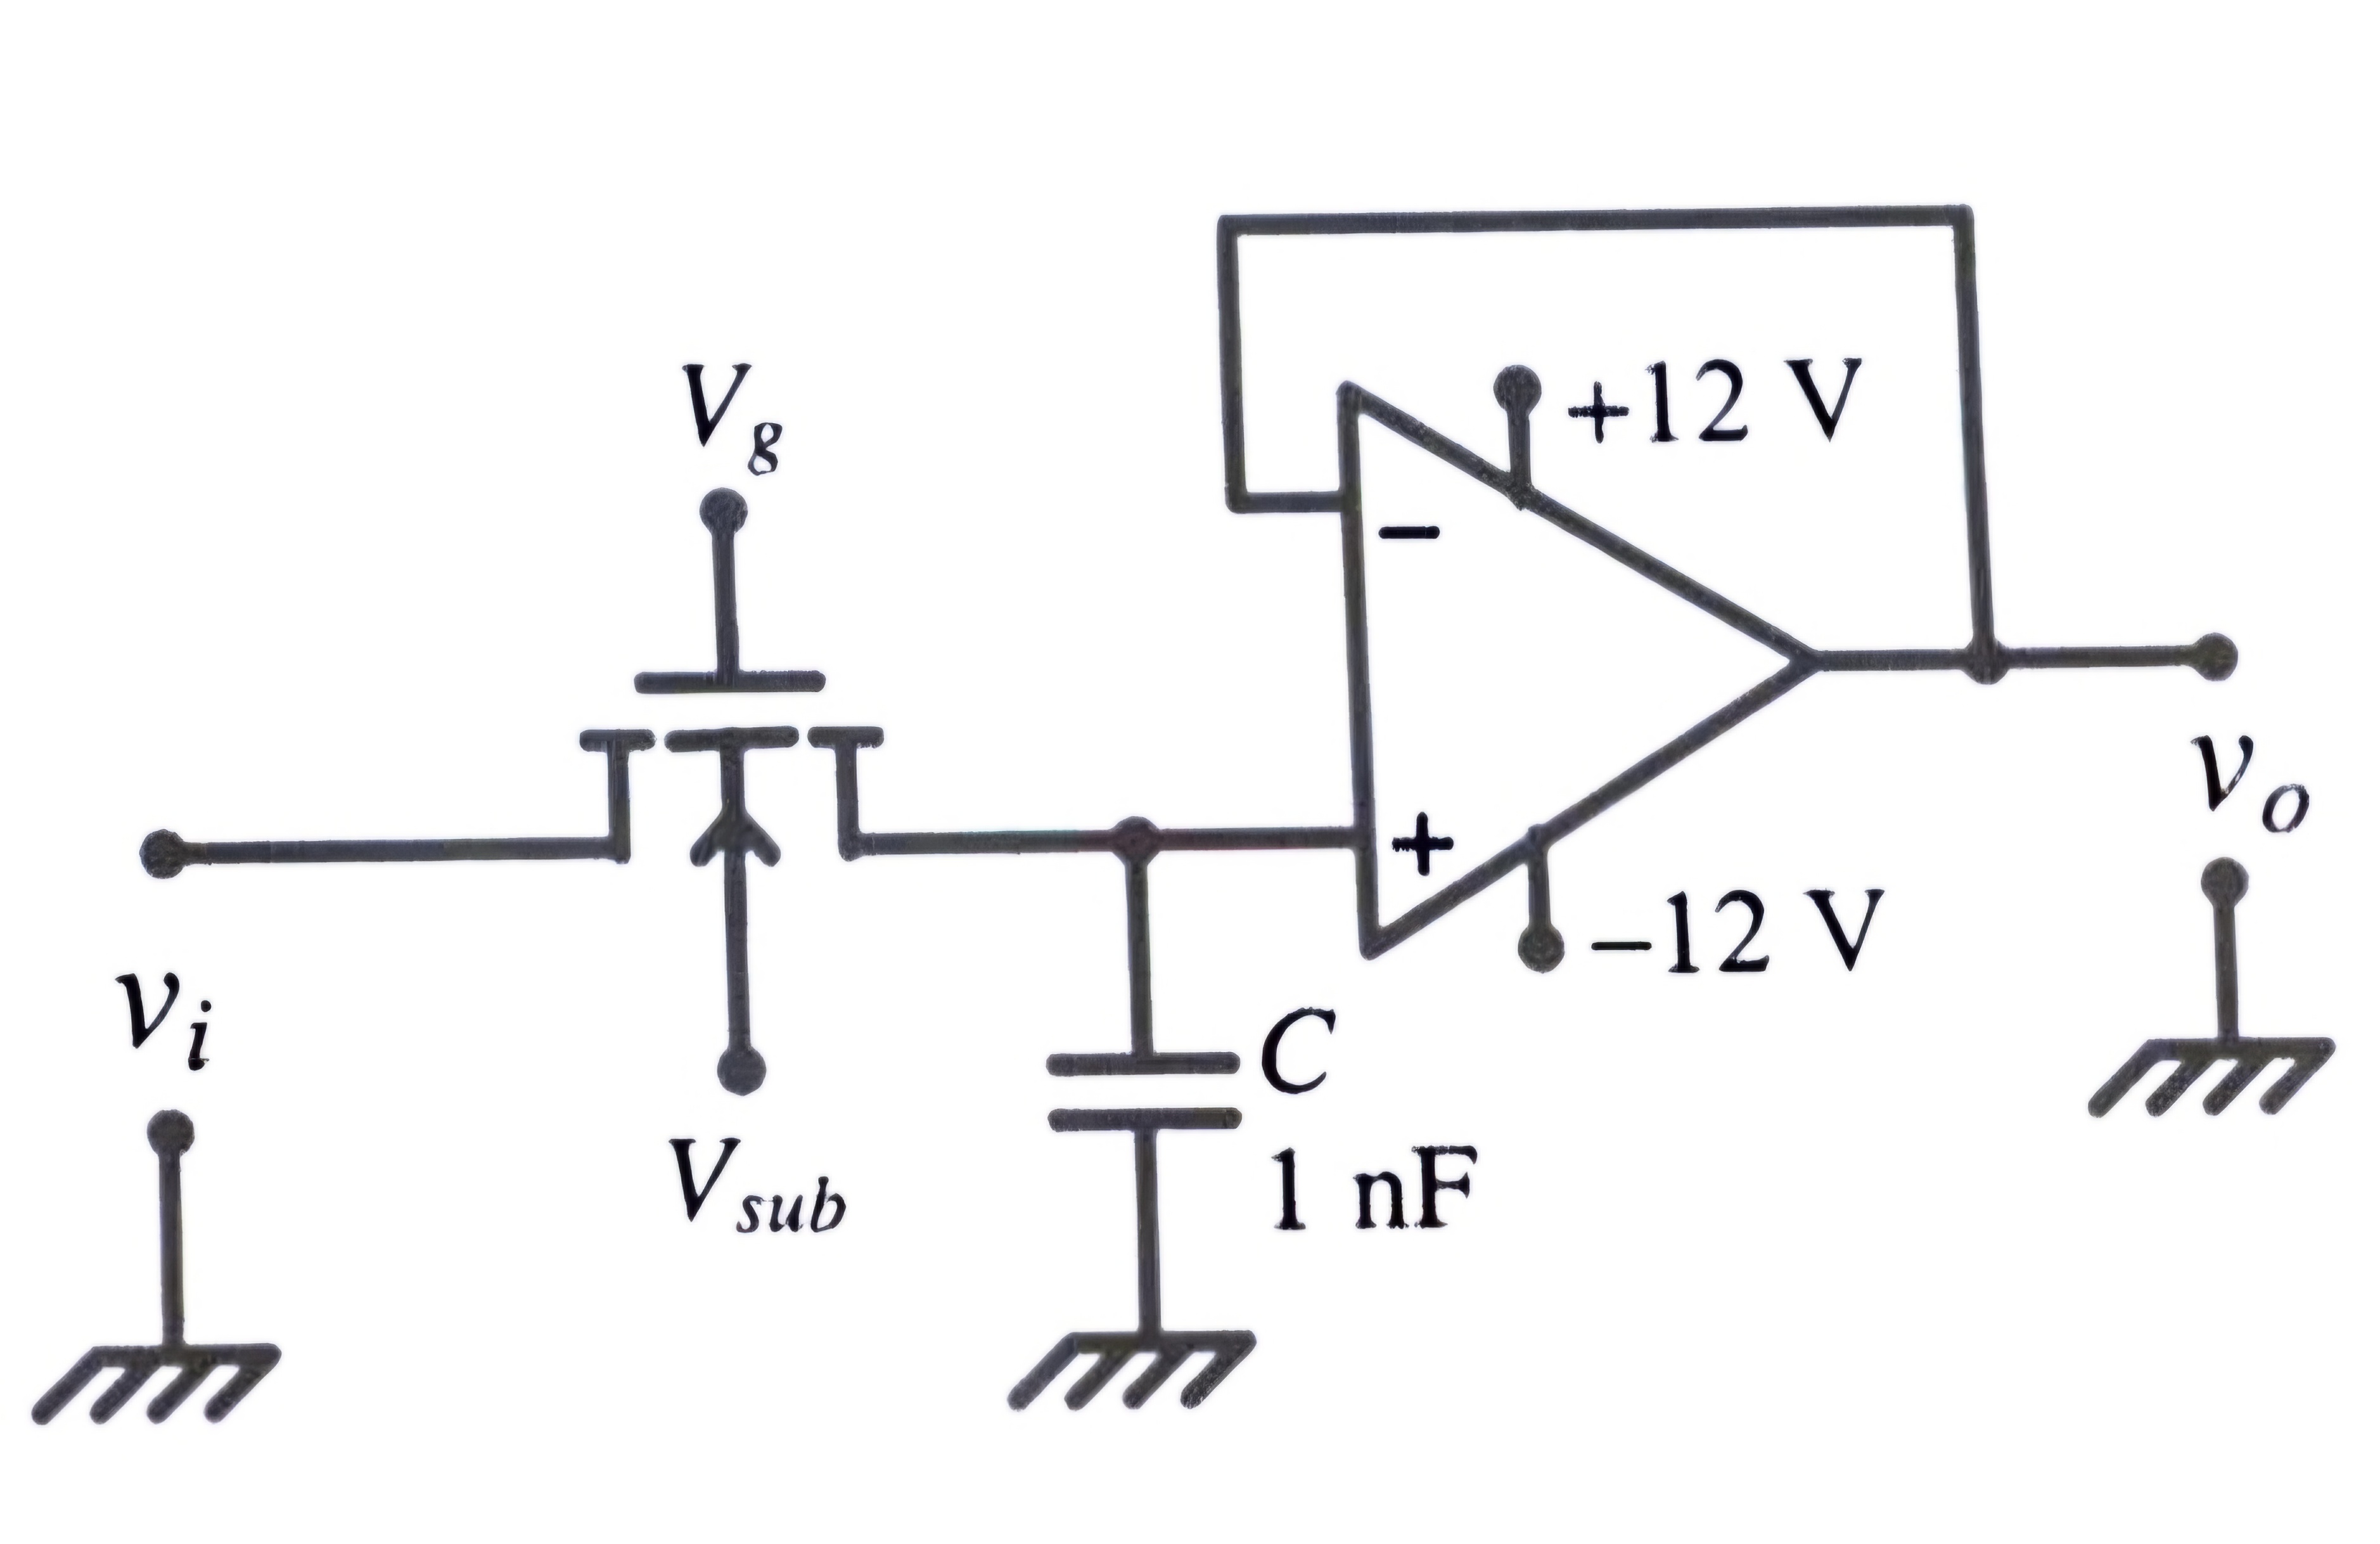
\includegraphics[width=0.5\columnwidth]{Figs/Q-51,52.jpg}
    \caption{Sample-and-Hold Circuit}
    \label{fig:placeholder_15}
\end{figure}

 

%51
\item The input voltage $v_i$ ranges from $-5\text{V}$ to $+5\text{V}$. Appropriate values of $V_{sub}$, of $V_g$ during sampling, and of $V_g$ during hold are, respectively \par \hfill{\brak{\text{GATE IN 2009}}}
\begin{enumerate}
    \begin{multicols}{2}
        \item $+12\text{V}$, $\ge+7\text{V}$, and $\le-3\text{V}$
        \item $-12\text{V}$, $\ge+3\text{V}$, and $\le-7\text{V}$
        \item $+12\text{V}$, $\ge+3\text{V}$, and $\le-7\text{V}$
        \item $-12\text{V}$, $\ge+7\text{V}$, and $\le-3\text{V}$
\end{multicols}
\end{enumerate}

%52
\item The circuit is used at a sampling rate of $1{\text{kHz}}$, with an A/D converter having a conversion time of $200{\mu}\text{s}$. The op amp has an input bias current of $10\text{nA}$. The maximum hold error is \par \hfill{\brak{\text{GATE IN 2009}}}
\begin{enumerate}
    \begin{multicols}{4}
        \item $1\text{mV}$
        \item $2\text{mV}$
        \item $5\text{mV}$
        \item $10\text{mV}$
    \end{multicols}
\end{enumerate}

 

\textbf{Common Data for Questions $53$ and $54$:}\par
The circuit shown in \figref{fig:placeholder_16} uses three identical transistors with $V_{BE}=0.7\text{V}$ and $\beta=100$. \par
Given $R_1=R_2=R_3=1\text{k}\ohm$, $kTlq_e=25\text{mV}$. The collector current of transistor $Q_3$ is $2\text{mA}$. 
\begin{figure}[H]
    \centering
    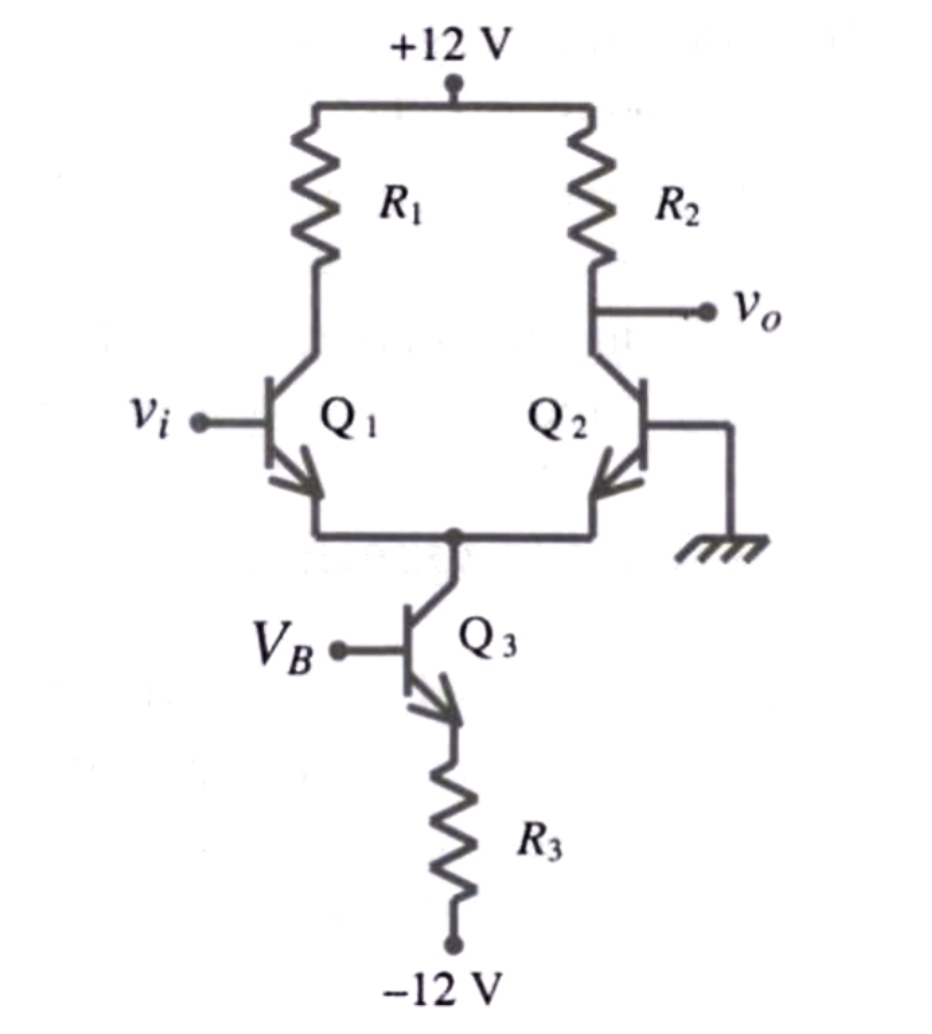
\includegraphics[width=0.5\columnwidth]{Figs/Q-53,54.jpg}
    \caption{Circuit Diagram}
    \label{fig:placeholder_16}
\end{figure}

%53
\item The bias voltage $V_B$ at the base of the transistor $Q_3$ is approximately \par \hfill{\brak{\text{GATE IN 2009}}}
\begin{enumerate}
    \begin{multicols}{4}
        \item $-9.3\text{V}$
        \item $-10\text{V}$
        \item $-10.3\text{V}$
        \item $-11.0\text{V}$
    \end{multicols}
\end{enumerate}

 

%54
\item The small-signal voltage gain of the circuit is \par \hfill{\brak{\text{GATE IN 2009}}}
\begin{enumerate}
    \begin{multicols}{2}
        \item $20$
        \item $-40$
        \item $20$
        \item $40$
    \end{multicols}
\end{enumerate}

 

\textbf{Common Data for Questions $55$ and $56$:}

 \figref{fig:placeholder_17} shows an arrangement for measuring small angular displacements in a vertical plane. A non-conducting tube of length $2l$ and rectangular cross section (width $w$, height $d$) is bent along an arc of a circle with radius $R>>>d$ centered at P. Four electrode plates of length $l$ and width $w$ are placed to form two curved parallel plate capacitors $\mathrm{C_1}$ and $\mathrm{C_2}$  with a negligible gap between them. The tube contains water with an air bubble of rectangular cross section (width $w$, height $d$) and length $l/4$. The capacitors are connected in a bridge circuit as shown in the figure, where the bridge has ac excitation $\nu_i$. Angular displacement $\Delta\theta$ occurs about the point P.

 \begin{figure}[H]
    \centering
    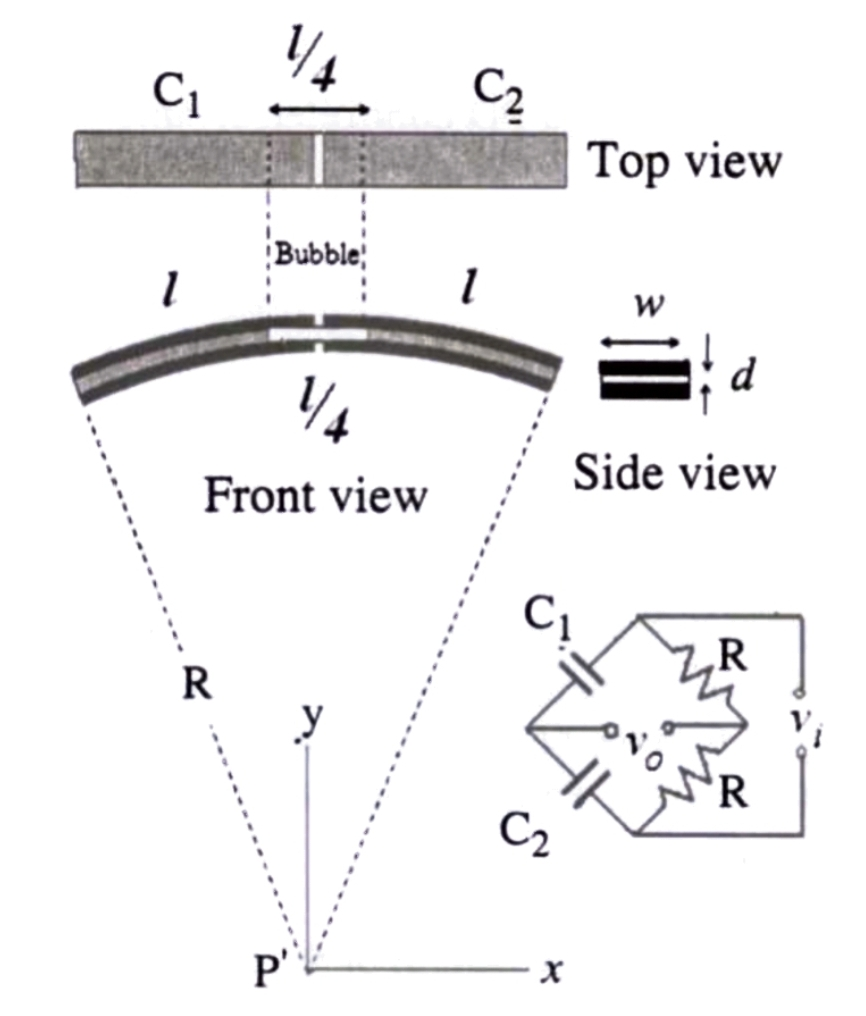
\includegraphics[width=0.5\columnwidth]{Figs/Q-55,56.jpg}
    \caption{Setup for measuring small displacements in vertical plane}
    \label{fig:placeholder_17}
\end{figure}

 

%55
\item The range of angular displacement (in radians) this system can measure is \par \hfill{\brak{\text{GATE IN 2009}}}
\begin{enumerate}
    \begin{multicols}{2}
        \item {$-\frac{l}{8R}$ to $+\frac{l}{8R}$}
        \item $-\frac{l}{4R}$ to $+\frac{l}{4R}$
        \item $-\frac{3l}{4R}$ to $+\frac{l}{4R}$
        \item $-\frac{l}{R}$ to $+\frac{l}{R}$
    \end{multicols}
\end{enumerate}

 

%56
\item The sensitivity {${\frac{v_o/v_i}{\Delta\theta}}$} is \par \hfill{\brak{\text{GATE IN 2009}}}
    \begin{enumerate}
        \item inversely proportional to $R$ and $l$
        \item inversely proportional to $R$ and directly proportional to $l$
        \item directly proportional to $R$ and $l$
        \item directly proportional to $R$ inversely proportional and $l$
    \end{enumerate}

\section*{\textbf{Linked Answer Questions}}
 

\textbf{Statement for Linked Answer Questions $57$ and $58$:}
 

A disturbance input $d\brak{t}$ is injected into the unity feedback control loop shown in \figref{fig:placeholder_18}. Take the reference input $r\brak{t}$ to be a unit step. 

\begin{figure}[H]
    \centering
    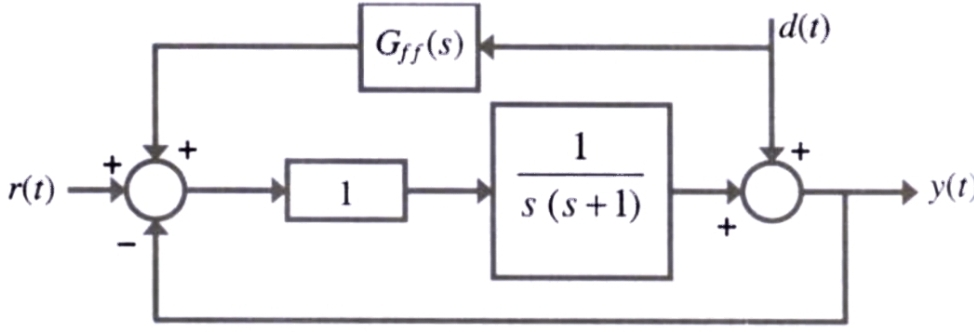
\includegraphics[width=0.5\columnwidth]{Figs/Q-57,58.jpg}
    \caption{For Questions 57 and 58}
    \label{fig:placeholder_18}
\end{figure}
 

%57
\item If the disturbance is measurable its effect on the output can be minimized significantly using a feedforward controller $G_{f f}\brak{s}$. To eliminate the component of the output due to $d\brak{t}=sint$, $G_{ff}\brak{j\omega}|_{\omega=1}$ should be \par \hfill{\brak{\text{GATE IN 2009}}}
\begin{enumerate}
\begin{multicols}{4}
    \item $\frac{1}{\sqrt2}\angle-\frac{3\pi}{4}$
    \item $\frac{1}{\sqrt2}\angle\frac{\pi}{4}$
    \item ${\sqrt2}\angle\pi$
    \item ${\sqrt2}\angle-\frac{\pi}{4}$
\end{multicols}
\end{enumerate}

%58
\item Let $G_{ff}\brak{s}$ be a PD controller. If $d\brak{t}=sin2t$, the amplitude of the frequency component of $y\brak{t}$ due to $d\brak{t}$ \par \hfill{\brak{\text{GATE IN 2009}}}
\begin{enumerate}
\begin{multicols}{4}
    \item $\sqrt{\frac{5}{13}}$
    \item $\sqrt{\frac{9}{13}}$
    \item $\sqrt{\frac{17}{13}}$
    \item $\sqrt{\frac{20}{13}}$
\end{multicols}
\end{enumerate}

 

\textbf{Statement for Linked Answer Question $59$ and $60$:} \par
 
A Michelson interferometer illuminated with a source of central wavelength $\lambda_0$ and spectral width $\Delta\lambda$  is adjusted for equal path difference for the beams returning from the two mirrors. When one of the mirrors is moved by a distance of $0.1\text{mm}$ from this position, $300$ fringes move past the field of view. When the mirror is moved further, the fringes completely disappear when the mirror is approximately $4\text{cm}$ from the initial position.

 

%59
\item The central wavelength of the source is \par \hfill{\brak{\text{GATE IN 2009}}}
\begin{enumerate}
\begin{multicols}{4}
    \item $540\text{nm}$
    \item $632.8\text{nm}$
    \item $667\text{nm}$
    \item $720\text{nm}$
\end{multicols}    
\end{enumerate}

 

%60
\item The spectral width of the source $\Delta\lambda$ is approximately \par \hfill{\brak{\text{GATE IN 2009}}}
\begin{enumerate}
\begin{multicols}{4}
    \item $0.0056\text{nm}$
    \item $0.0100\text{nm}$
    \item $0.0500\text{nm}$
    \item $0.1000\text{nm}$
\end{multicols}    
\end{enumerate}

 

 
\end{enumerate}


\end{document}
